\documentclass[a4paper,10pt]{article}
\usepackage{listings}
\usepackage{graphicx}
\usepackage{amssymb}
\lstset{language=C}
\author{Federico Mariti}
\title{Progetto del modulo di Laboratorio di Programmazione
  Concorrente di Sistema, corso~A, a.a. 2009/10}
\date{}
\begin{document}
\maketitle
\renewcommand{\contentsname}{Indice}
\setcounter{tocdepth}{2}
\tableofcontents
\newpage
\section{Organizzazione del codice}
Tutti i file sorgenti dei programmi \texttt{msgserv}, \texttt{msgcli}
e dei programmi di test sono posizionati nella directory
\verb+PROJ_BASEDIR/src/+. Oltre alla libreria \texttt{msg} sono state
implementate altre due librerie: \texttt{blockingCollection} e
\texttt{threadPool}. 

La libreria \texttt{blockingCollection} dovrebbe contenere un insieme
di tipi di dato astratti che realizzano strutture dati di utilit\`a
con la caratteristica di fornire, nelle funzioni di manipolazione di
tali oggetti\footnote{Per ``oggettto'' si intede tipo di dato
  astratto, passivo (una struttura dati) o attivo (capacit\`a di
  autocontrollo)}, sincronizzazione implicita ed esplicita dei threads
che ne fanno uso. In realt\`a tale libreria contine solo l'oggetto
``\texttt{blockingList}'' implementato come elementi (nodi)
linkati. Tale struttura dati \`e molto usata nello svolgimento del
progetto come pila/coda per realizzare l'interazione tra pi\`u threads
secondo il modello \emph{produttore-consumatore}.

La libreria \texttt{threadPool} realizza un oggetto esecutore di un
insieme di attivit\`a (task) asincrone sottomesse usando un insieme
arbitrario di threads. Tale oggetto provvede a risolvere due problemi
spesso ricorrenti in un processo ``servente'':
\begin{itemize}
  \item Fornisce un limite superiore alle risorse (threads) utilizzate
    durante l'esec\-uzione dell'insieme di compiti sottomessi;
  \item In generale, rispetto ad una gestione esplicita dei thread,
    migliorano le prestazioni durante l'esecuzione di un numero
    elevato di task sottemessi, in quanto i threads del pool sono
    riutilizzati per l'esecuzione di pi\`u attivit\`a sottomesse in
    modo da non pagare il costo (elevato) di creazione ed avvio di un
    thread per ogni esecuzione di un task sottomesso.
\end{itemize}
Per tali caratteristiche questo oggetto \`e usato nell'implementazione
del programma \texttt{msgserv} per sottomettere la gestione di una
nuova connessione a nuovi threads. Tuttavia l'implemntazione
``da~zero'' di un tale oggetto \`e motivata piuttosto da fini
didattici che effettiva esigenza in quanto le caratterstiche sopra
descritte sarebbero agilmente ottenibili (pi\`u semplicemente) con una
stutturazione ad-hoc per il programma dei threads e delle strutture
dati che compongono un thread pool. Inoltre molte caratterische del
thread pool non sono usate e pertanto non implementate o testate, \`e
tuttavia fornita una valida interfaccia (i prototipi delle funzioni e
specifiche) e definizioni i tipi necessari (come l'oggetto per
memorizzare il risultato pendente di un task). 

Per quanto riguarda i tipi di dato astratto implementati e non
richiesti dal progetto \`e stata fornita una implementazione che
nasconde l'implementazione fornendo all'utente solo i prototipi delle
funzioni pubbiche con cui utilizzare gli oggetti in questione. Ci\`o
non permette una allocazione di uno di questi oggetti in memoria stack
in quanto non \`e nota la dimensione della struttura che descrive
l'oggeto. Per tale motivo non sono stati modificati gli oggetti
\texttt{genList} e \texttt{genHashTable} richiesti dal progetto.

%%%%%%%%%%%%%%%%%%%%%%%%%%%%%%%%%%%%%%%%%%%%%%%%%%%%%%%%%%%%%%%%%%%%%%%%

\section{Tipi di Dati Astratti implementati}
I tipi di dati astratti passivi implementati rappresentano strutture
dati quali \emph{liste} e \emph{tabelle hash}. \`E stato inoltre
implementato il tipo di dato astratto \emph{thread pool} che
rappresenta un esecutore di task (o attivit\`a) asincroni tramite un
insieme di thread opportunamente gestito. Un elenco dei tipi di dato
significativi implementati:
\begin{description}
  \item[list\_t] lista generica di coppie (chiave, valore)
  \item[hashTable\_t] tabella hash generica
  \item[blockingList\_t] lista generica bloccante
  \item[threadPool\_t] esecutore di task asincroni secondo il modello a
    pool
\end{description}
Per garantire la propriet\`a di \emph{information hiding} sui tipi di
dato astratto, l'imple\-mentazione di questi \`e strutturata in due
file header e in uno o pi\`u file sorgenti. Il primo file header
prende il nome del tipo di dato astratto e contiene la dichiarazione
delle funzioni \emph{pubbliche} che agiscono sull'oggetto e la
definizione di macro di utilit\`a. Il secondo file header prende il
nome del tipo di dato seguito da ``\_private'' e contiene la
definizione delle strutture che implementano il dato ed altre
informazioni \emph{riservate} alla sola implementazione del dato e non
necessarie all'utente. All'utente vengono forniti il file header
pubblico e la libreria, cos\`i da nascondere le scelte implementative
del tipo di dato. La scelta di garantire tale propriet\`a e fornire
delle valide interfaccie \`e motivata dal fatto per cui l'uso di un
oggeto tramite l'accesso diretto ai campi delle strutture che lo
costituisco pu\`o provocare comportamenti non attesi/definiti in
generale e soprattutto nel caso in cui venga cambiata
l'implementazzione del tipo di dato astratto.

Per quanto riguarda le strutture quali liste e tablla hash, per ogni
funzione $\mathnormal{f}$ che agisce sugli elementi della struttura
\`e definita (nell'header pubblico) una macro parametrica che
definisce un'altra funzione, wrapper di $\mathnormal{f}$, il cui
prototipo non ha riferimenti generici \texttt{void *} ma vengono
specificati i tipi passati come parametri alla macro. Il comportamento
della funzione wrapper \`e identico alla funzione generica. L'utilizzo
di tali macro \`e a discrezione dell'utente e se adeguato permette di
garantire alcune propriet\`a aggiuntive, quali:
\begin{itemize}
  \item warining di tipo a tempo di compilazione nell'invocazione non
    corretta di una funzione;
  \item utilizzo di una lista o tabella hash con elementi aventi
    valori (e chiavi) di tipo omogeneo;
  \item utilizzo di un sottoinsieme di funzioni per una lista che
    offere l'astrazzione di pi\`u modelli di manipolazione dati quali
    \textsc{lifo} (pile) e \textsc{fifo} (code).
\end{itemize}
Ad esempio per la funzione (in blockingList.h):
\begin{verbatim}
int blockingList_push(blockingList_t * l, void * valuep);
\end{verbatim}
sia ha (in blockingList.h) la macro:
\begin{verbatim}
#define define_blockingList_push(wrapperFunName, valuepType)   \ 
  int wrapperFunName(blockingList_t * l, valuepType valuep) {  \
    return blockingList_push(l, valuep);                       \
  }
\end{verbatim}
l'utente pu\`o usare tale macro nel proprio codice per definire una
funzione che agisce su una lista bloccante di interi, nel seguente
modo:
\begin{verbatim} 
...
#include "headerPath/blockingList.h"
define_blockingList_push(myIntList_push, int)
...
{
  blockingList_t * myList = 
    blockingList_new(0, copy_int, cmpr_int);
  myIntList_push(myList, 123);
  ...
}
...
\end{verbatim}

\subsection{Generic List}
Lista di coppie (chiave, valore), entrambi gli elementi della lista
sono di tipo generico. 

Non \`e \emph{thread-safe}. Accessi e manipolazioni da parte di pi\`u
thread concorrenti sulla stessa lista provocano comportamenti non
prevedibili.

Usata per implementare le liste di collisione nella tabella hash
generica.

\subsection{Generic Hash Table}
Una tabella hash di chiavi e valori generici. Il probblema delle
collisioni di chiavi con stessa indice hash \`e risolto con le liste
di collisione. Non \`e implementato il ridimensionamento della tabella
in base al fattore di carico.

Non \`e \emph{thread-safe}. Accessi e manipolazioni concorrenti della
stessa tabella provocano comportamenti non prevedibili, per tali
situzioni \`e necessario assicurare la mutua esclusione nelle
operazioni che modificano la struttura interna della tabella.

Usata per implementare la tabella degli utenti autorizzati nel
processo \texttt{msgs\-erv}.

\subsection{Blocking List}
Lista bloccante di elementi con tipo qualsiasi ed eventualmente
disomogenei. Con il termine bloccante si intende che le funzionait\`a
di estrazione di un valore da tale struttura sono caratterizzate
dall'attesa che la lista sia non vuota, e le operazioni di inserzione
di un valore attendono la disponibilit\`a di spazio nella
lista. L'implementazione \`e garantita \emph{thread-safe} ovvero,
tutti i metodi che modificano la struttura interna della lista sono
eseguiti in modo atomico usando un lock interno o altre forme per
controllare l'esecuzione concorrente del codice.

Il modello usato per garantire la correttezza in caso di un uso
concorrente dell'oggetto \`e quello tipico Java: la struttura dati
bloccante (la lista in questo caso) contine un lock di tipo
\texttt{pthread\_mutex\_t} per garantire l'uso esclusivo dell'oggetto
e un singolo monitor di tipo \texttt{pthread\_cond\_t} per realizzare
la coda sulle due condizioni ``lista non vuota'' e ``spazio
disponibile'' e i meccanismi di sospensione e sveglia. Attualmente il
lock non \`e ricorsivo, ne prevede il controllo sull'identificatore
del thread, tali caratteristiche non sono necessarie ai fini del
progetto, ma possono essere agilmente sviluppate in un secondo momento
vista la caratteristica di \emph{information hiding} di tale struttura
dati, creando un nuovo tipo di dato wrapper di
\texttt{pthread\_mutex\_t}, che ne utilizzi ed estenda le
funzionalit\`a, tale tipo di dato verr\`a usato per realizzare il lock
interno alla lista.

L'interfaccia pubblica ovvero le funzioni e le macro con le quali
l'utente adopera la struttura dati, \`e definita nell'header
\texttt{blockingList.h}, le strutture che costituiscono la lista sono
invece definite nell'header \texttt{blockingList\_private.h} non
visibilie all'utente. L'interfaccia pubblica prevede solo la
definizione del tipo di dato \texttt{blockingList\_t} e la
dichiarazione delle funzionini con le quali adoperare la struttura.

L'iterazione degli elementi di tale lista pu\`o essere effettuata con
il corrispondente tipo di dato iteratore \texttt{blockingList\_itr\_t}
definito nell'header pubblico \texttt{blockingList\_itr.h} il quale
definisce i classici metodi per iterare la lista.

Le funzioni \texttt{blockingList\_lock} e
\texttt{blockingList\_unlock} presenti nell'header pubblico della
lista assicurano l'accesso esclusivo alla lista e a tutte le
funzionalit\`a per un blocco di codice arbitrario. Occorre porre
attenzione al fatto che (attualmente) il mutex della lista non \`e
ricorsivo, quindi l'invocazione di una funzionalit\`a che richieda
l'accesso esclusivo alla lista, successiva ad una chiamata del lock
esplicito causer\`a un \emph{dead-lock}. Tali funzioni di lock e
unlock sono comunque utilizzabili per accedere esclusivamente alla
lista durante una iterazione della stessa.

Tale oggetto \`e spesso usato per effettuare la comunicazione tra
thread dello stesso processo nell'implementazione del programma
\texttt{msgserv} e del tipo di dato astratto \texttt{threadPool\_t}

\subsection{Thread Pool}
Esecutore di attivit\`a asincrone, con e senza valore di ritorno,
tramite un insieme di threads lavoratori opportunamente
autogestito. Tali threads sono in grado di eseguire in sequenza pi\`u
task sottomessi al thread pool cos\`i da minimizzare il costo di
overhead dovuto alla creazione di un thread rispetto ad una gestione
esplicita dei threads. Le politiche di gestione dell'insieme dei
threads sono due:
\begin{description}
  \item[fixed] \`e fissata la dimensione massima e minima dell'insieme
    dei thread;
  \item[cached] il tempo di inattivit\`a dei threads \`e limitato.
\end{description}
I threads che costituiscono tale tipo di dato astratto sono solamente
i thread lavoratori (attivi o meno), non esiste un thread
dispatcher. L'insieme dei threads lavoratori pu\`o variare nel tempo
se \`e stato fornito un tempo massimo di inattivit\`a dei threads o in
seguito all'invocazione di una funzionalit\`a quali
\texttt{threadPool\_submit}, \texttt{threadPool\_shutdown*}. 

Se fissata una dimensione massima del pool di threads, un task
sottomesso non viene eseguito immediatamente ma \`e inserito in una
coda, in attesa che un thread attivo termini l'esecuzione di un task
sottomesso precedentemente. Ad ogni modo, indipendentemente dal tipo
\emph{fixed} o \emph{cached} del thread pool, l'attivit\`a di un thread
lavoratore \`e eseguire ciclicamente l'attesa di un nuovo task dalla
coda dei task sottomessi ed eseguire l'attivit\`a ed eventualmente (se
richiesto) salvare il risultato. La coda dei task \`e implementata con
un oggetto \verb+blockingList_t+, in modo da garantire la correttezza
nell'accesso concorrente alla lista e realizzare l'attesa passiva di
un nuovo task.

La terminazione del thread pool \`e implementata in due modi: 
\begin{itemize} 
  \item Aggiungendo uno speciale task in coda alla lista dei task
    sottomessi. Tale task non fa altro che invocare la funzione
    \texttt{pthread\_exit((void *) 0)}. In tal modo viene realizzata la
    terminazione graduale del thread pool (vedi specifiche di
    \verb+threadPool_shutdown}+;
  \item Cancellando tutti i thread o tutti i thread non attivi. In
    questo modo viene implementata la terminazione itantanea o la
    terminazione ``finisci l'esecuzione'', vedi le specidiche di
    \verb+threadPool_shutdownNow+ e
    \texttt{threadPo\-ol\_shutdownDoActive});
\end{itemize}

%%%%%%%%%%%%%%%%%%%%%%%%%%%%%%%%%%%%%%%%%%%%%%%%%%%%%%%%%%%%%%%%%%%%%%%%

\section{Struttura del Server}
\subsection{Strutture dati usate e condivisione delle stesse tra i threads}
Vengono elencate e brevemente descritto lo scopo delle strutture dati
usate; nei pargrafi successivi vengono approfonditi e motivati gli usi
di tali oggetti, in particolare di quelli non menzionati nelle
specifiche/consegna del progetto.
\begin{description}
  \item [Thread Pool] per servire le richieste dei clienti connessi;
  \item [Tabella degli utenti (autorizzati)] mantenere lo
    stato \{``connesso'', ``non connesso''\} degli
    utenti e la coda dei messaggi in uscita verso l'utente, se
    quest'ultimo \`e connesso;
  \item [Lista degli utenti connessi] per mantenere l'elenco degli
    utenti connessi, in modo da non dover iterare tutta la tabella
    degli utenti ad ogni richiesta della lista delgi utenti da parte
    di un client;
  \item [Pila dei messaggi di log]
  \item [Coda dei messaggi in uscita su una connessione] una per
    utente connesso.
\end{description}
Le strutture \{ThreadPool, Tabella utenti, Lista utenti connessi, Pila
messaggi log\} sono create in fase di inizializzazione del processo e
sono riferite da una variabile dichiarata in ambiente globale, quindi
tali oggetti sono condivisi tra tutti i thread del processo. La \{Coda
di messaggi in uscita\} invece viene creata solo alla connessione di
un utente (il nome) alla chat, tale struttura viene riferita nella
Tabella utenti, perci\`o viene condivisa tra tutti i thread del
processo.

\subsection{I threads del processo}
Di seguito vengono chiamati \emph{worker-thread} i thread del processo
\texttt{msgserv} la cui attivit\`a \`e caratterizata dal servire le
richieste di uno o pi\`u utenti connessi. Un worker-thread pu\`o
essere associato, ovvero servire, una sola o pi\`u (tutte) connessioni
a seconda della stuttura che si vuole dare al server. Un worker-thread
sar\`a chiamato \emph{scrittore} (mittente) o \emph{lettore}
(ricevente) a seconda del servizio che svolge sulla connessione a cui
\`e associato.

Si \`e scelto di strutturare il server in modo tale per cui ogni
connessione ha \emph{associati} due worker-thread, uno lettore e
l'altro scrittore; per \emph{associato in lettura/scrittura} si
intentde (ora ed in futuro) che la connessione \`e servita in
letttura/scrittura \emph{unicamente} dal worker-thread corrispondente;
l'\emph{invio} di un messaggio unicast/broadcast che un worker-thread lettore
riceve dal rispetivo utente \`e implementato con la comunicazione del
thread lettore stesso con il worker-thread scrittore associato alla
connessione dell'utente destinatario. Le motivazioni di tale
strutturazione sono date nel paragrafo \textbf{(3.5)}. Il processo
\texttt{msgserv} \`e quindi formato dall'insieme dei worker-thread di
cardinalit\`a doppia al numero di connessioni, dal thread scrittore
sul file di log e dal thread principale o dispatcher.

La vita dei thread dispatcher e scrittore sul file di log corrsiponde
alla vita del processo. I worker-thread sono gestiti dall' oggetto
Thread pool quindi possono eseguire pi\`u attivit\`a nella loro vita,
nello specifico possono esssere riceventi o scrittori di pi\`u utenti;
la vita di un worker-thread dipende dal Thread pool se \`e prevista un
morte a causa di inattivit\`a. 

Le attivit\`a (task) che descrivono i thread di tale processo hanno in
comune il modello ``servente'' che prevede tre fasi:
\begin{description}
  \item[Inizializzazione] di strutture dati e variabili;
  \item[Servire la prossima richiesta] fino alla terminazione del
    thread viene reperita una richiesta sottomessa da un cliente e
    viene servita;
  \item[Terminzione] vengono liberate le risorse e vengono effettualte
    le ultime interazioni con altri thread.
\end{description}
Ovviamente la definizione di ``terminazione'', ``cliente'' ed ``interazione con
il cliente o altro thread'' varia a seconda dell'attivit\`a .

Lo scopo del thread dispatcher \`e di inizializzare le principali
strutture dati, avviare il thread scrittore dei messaggi di log e
restare in attesa di richieste di connessione sul socket di ascolto
collegato al path prestabilito. Dopo aver stabilito una
connessione\footnote{Trattasi di connessione logica tra i due processi
  secondo l'internal protocol di UNIX, non la connessione di un utente
  (il nome) alla chat.} con un cliente viene sottomesso alla struttura
threadPool il compito di eseguire il task del worker-thread lettore
con argomento il file descriptor del socket attivo appartenente alla
nuova connessione. Tale nuovo worker-thread ha il compito iniziale di
attendere il messaggio di login contenente il nome utente del cliente
secondo il protocollo definito in \texttt{comsock.h} e nelle specifice
del progetto, e di verficare l'autenticazione di tale nome. Solo dopo
l'autenticazione, l'utente si considera collegato alla chat, il
worker-thread lettore procede a creare una coda dei messaggi e
impostarla nella Tabella utenti autorizzati al nome utente
ricevuto. Tale coda rappresenta i messaggi in uscita verso l'utente ed
\`e passata come argomento, con il file descriptor del socket
appartenente alla connessione, ad un nuovo worker-thread scrittore il
cui task \`e sottomesso al threadPool dallo stesso worker-thread
lettore. Prima di iniziare a ricevere messaggi dall'utente, il
worker-thread lettore deve solo aggiungere il nome utente alla lista
degli utenti connessi. Il worker-thread scrittore creato da un lettore
dopo l'autenticazione di un utente ha il compito iniziale di inviare
la conferma di avvenuta connessione secondo il protocollo stabilito,
quinidi si mette in attesa di un messaggio disponibile nella coda dei
messaggi in uscita verso l'utente ricevuta come argomento. L'attesa di
un nuovo messaggio e' bloccante, una volta disponibile un messaggio
vengono effettuati controlli sul tipo del messaggio e sulla lunghezza
del buffer, quindi viene spedito all'utente. \`E quindi compito di
ogni worker-thread lettore, una volta ricevuto un messaggio di tipo
\{\textsc{to\_one}, \textsc{bcast}\} creare il o i messaggi da
sottmettere al o ai worker-threads scrittore e la o le stringhe da
sottomettere al thread scrittore dei messaggi di log. Come avvengono
tale sottomissioni di servizi interni al processo, ovvero come i
threads comunicano/cooperano, \`e descritto nei paragrafi successivi.

\subsection{Comunicazione e sincronizzazione tra threads}
L'interazione tra threads avviene tramite risorse condivise quali pile
o code. In generale tali risorse o ``canali di comunicazione'' hanno
\begin{math} n \geq 1 \end{math} threads produttori e \begin{math} m
  \geq 1 \end{math} threads consumatori, \`e pertanto necessario
imporre vincoli ai threads stessi per quanto riguarda la competizione
alle risorse condivise e la cooperazione. Ci\`o \`e effettuato (nella
maggior parte dei casi) in modo trasparente usando la struttura dati
bloccante \texttt{blockingList\_t} descritta nel paragrafo
\textbf{(2.3)} che incapsula oggetti lock e monitor cos\`i da
garantire le propriet\`a di mutua esclusione sull'oggetto e di
cooperazione tra threads. Fa eccezione la risorsa Tabella utenti
autorizzati la quale, in generale, \`e acceduta in scrittura da pi\`u
worker-threads; tali threads, quindi, necessitano del vincolo di mutua
esclusione nell'accesso alla tabella. Tale vincolo non \`e fornito
dalla struttura dati \texttt{hasTable\_t} che realizza la tabella ma
\`e garantito esplicitamente da un lock di tipo
\texttt{pthread\_mutex\_t} dichiarato \texttt{static} in una funzione
visibile a tutti i thread del processo. Tale funzione permette di
inizializzare, bloccare, sbloccare e distruggere il mutex, inoltre
garantisce propriet\`a aggiuntive in modo da avere il ritorno di
errori piuttosto che comportamenti non attesi (vedi documentazione).

\subsection{Scrittura dei messaggi di log in logfile}
Il compito di eseguire la scrittura dei messaggi sul file di log viene
effettuta da un unico thread specializzato a fare ci\`o. Un messaggio
letto da un socket vine scritto sul file di log grazie all'interazione
tra il worker-thread lettore che ha ricevuto la richiesta di invio del
messaggio e tale thread. La comunicazione tra questi due threads
avviene tramite una pila (bloccante), l'uso di una struttura
\textsc{lifo} \`e motivato dalla fatto che non \`e richiesto l'ordine
in cui i messaggi compaiono nel file e dal breve tempo (il minimo
possibile) di inserzione di un messaggio da parte di un worker-thread
lettore. Si nota che il tempo minimo di inserzione sarabbe disponibile
anche con un'ordinazione \textsc{fifo} su una coda a due teste;
implementare un tale struttura dati \`e un possibile upgrade in quanto
torna utile nella comunicazione dei worker-thread lettori e scrittori,
dove \`e necessario un ordinamento \textsc{fifo} dei messaggi inviati.

\subsection{Invio di messaggi su una connessione}
L'invio di un messaggio, da parte di un worker-thread, ad un utente
richiede la scrittura di tale messaggio nel socket attivo
corrsipondente alla connessione dell'utente, tale scrittura non deve
essere interrotta da scritture di altri worker-thread che eseguono
l'invio di un messaggi. Si pu\`o pensare a due strutturazioni dei
worker-thread che risolvono tale problema in due modi diversi:
\begin{itemize}
  \item un qualsiasi socket attivo \`e scritto da un unico
    worker-thread. Un worker-thread che esegue l'invio di un messaggio
    deve interagire con il worker-thread associato alla connessione
    destinataria. L'interazione tra threads avviene come descritto nel
    paragrafo \textbf{(3.3)};
  \item un qualsiasi socket attivo pu\`o essere scritto da un numero
    arbitrario di worker-thread (tutti), ovvero un qualsiasi
    worker-thread pu\`o scrivere direttamente sul socket attivo
    destinatario. Occorre garantire la mutua esclusione nella
    scrittura su diun socket da parte dei worker-thread.
\end{itemize}
Di seguito vengono analizzate alcune soluzioni a tale problema per
motivare la scelta fatta.

\subsubsection{Unico thread scrittore}
Disporre di un solo thread che esegue l'invio di un messaggio,
reperito da un worker-thread, in un socket qualsiasi. La comunicazione
tra tale thread ed i worker-thread avviene tramite una lista condivisa
di coppie (messaggio,~file-descriptor~socket).
\begin{description}
  \item[contro:] Tale strutturazione pecca in efficenza in quanto si
    ha un collo di bottiglia nella sottomissione dei messaggi da
    inviare dai worker-thread al solo thread scrittore, pertanto tale
    soluzione viene scartata.
\end{description}

\subsubsection{Due worker-thread per ogni connessione}
Per ogni connessione (socket) sono associati due worker-thread, un
ricevente (lettore) ed uno mittente (scrittore) di messaggi. Quando un
thread ricevente desidera inviare un messaggio su una connessione
qualsiasi (a causa di una richiesta d'invio unicast o bradcast
ricevuta dall'utente associato) tale spedizione viene sottomessa al
worker-thread mittente associato alla connessione destinataria
aggiungendo il messaggio alla coda condivisa dei messaggi in uscita
sulla connssione.
\begin{description}
  \item[pro:] reattivit\`a del worker-thread lettore nel servire le
    richieste dell'utente associato. L'intervallo di tempo tra due
    \verb+receiveMessage+ dal socket associato dipende
    solo\footnote{In realt\`a l'intervallo di tempo tra due receive
      \`e caratterizzato anche dal tempo di creazione del messaggio da
      spedire all'utente e da quello per creare la stringa da
      sottomettere al worker-thread che scrive sul file di log. Si
      vuole per\`o sottolineare il fatto che la spedizione di un
      messaggio da parte di un worker-thread lettore non dipende dal
      tempo di scrittura del messaggio stesso sulla connessione}
    dall'accesso esclusivo alla lista condivisa dei messaggi in uscita
    della connessione e dall'operazione di inserzione del messaggio da
    spedire, \emph{non} dipende invece dal tempo d'invio del
    messaggio;
  \item[contro:] uso di diverse risorse, in particolare il numero di
    worker-thread \`e doppio del numero degli utenti connessi.
\end{description}

\subsubsection{Un worker-thread per ogni connessione}
Ogni connessione (socket) ha associato un solo worker-thread, le
scritture e le letture da un socket sono eseguite esclusivamente dal
worker-thread associato. L'invio di un messaggio da un worker-thread
consiste nell'aggiungere il messaggio stesso nella lista dei messaggi
di uscita per la connessione dell'utente destinatario e iniviare un
segnale al worker-thread associato a tale connessione, in quanto
potrebbe essere bloccato in \verb+receiveMessage+.
\begin{description}
  \item[contro:] il server pu\`o essere poco reattivo rispetto alle
    richieste degli utenti, in quanto i worker-thread associati alle
    connessioni eseguono i due compiti di lettura e scrittura di
    messaggi, la scrittura di tutti i messaggi destinati ad una
    connessione puo' rallentare la ricezione dei messaggi dalla
    connessione stessa, soprattutto se vi sono molti utenti connessi e
    il tempo di scrittura \`e significativo.
\end{description}

\subsubsection{Mutua esclusione nella scrittura}
Esiste una corrispondenza uno-a-uno tra connessioni e worker-thread
\emph{solamente} per l'operazione di lettura. L'invio di un messaggio
\`e effettuato da un qualsiasi worker-thread invocando
\texttt{sendMessage} direttamente sul socket destinatario, dopo aver
ricevuto un messagggio \verb+TO_ONE+ o \verb+BCAST+ dalla connessione
associata. In tale strutturazione i worker-thread possono accedere
concorrentemente in scrittura ad uno stesso socket, ci\`o richiede il
verificare l'accesso esclusivo al soket per \emph{tutta} la durata di
spedizione del messaggio. Alune soluzioni:
\begin{description}
  \item[Un solo mutex per tutte le connessioni] tale soluzione e'
    implementabile usando una variabile \verb+pthread_mutex_t+ statica
    all'interno della funzione \texttt{sendMessage} della libreria
    \texttt{comsock.h} oppure globale ai worker-thread.
    \begin{description}
       \item[contro:] un unico punto di attesa per l'accesso esclusivo
         in scrittura ad una connessione qualsiasi, quindi possibili
         lunghe attese per la spedizione e di conseguenza bassa
         reattivit\`a del server nel sottomettere le richieste degli
         utenti.
    \end{description}
  \item[Write atomica] implementare la funzione \texttt{sendMessage}
  della libreria \texttt{comsock\-.h} im modo da effettuare una unica
  invocazione della funzione \texttt{write} sul socket della
  connessione di un oggetto di dimensioni inferiori di \\
  \begin{math}
    \verb+{PIPE_BUF}+ \geq \verb+{_POSIX_PIPE_BUF}+ = 512
  \end{math}
  \begin{description}
    \item[pro:] viene usata una propriet\`a
      dell'implementazione della system call \texttt{write} che
      solleva il programmatore dall'uso di strutture dati o modelli di
      interazione di threads per risolvere tale problema;
    \item[contro:] la dimensione dei messaggi e' fissata;
    \item[contro:] per garantire l'atomicit\`a dell'invio di un
      messaggio occore effettuare una sola invocazione della system
      call \texttt{write} quindi si deve disporre dei campi del
      messaggi memorizzati in modo sequenziale in memoria, cosa che
      non si ha in quanto (l'eventuale) campo \emph{buffer} \`e
      riferito indirettamente. \`E quindi necessario, nella funzione
      \texttt{sendMes\-sage} una allocazione della memoria heap pari
      alla dimensione del buffer pi\`u 5 byte per gli altri due campi
      e l'effetture la copia dei \emph{valori} dei tre campi.
  \end{description}
\item[Un mutex per ogni connessione] ad ogni connessione deve essere
  associato una variabile \verb+pthread_mutex_t+ per garantirne
  l'accesso esclusivo. Tale associazione pu\`o essere implementata con
  una hash table, ad esempio con la stessa user-table che definisce lo
  stato degli utenti connessi.
  \begin{description}
  \item[contro:] il tempo impiegato da un worker-thread per la
    scrittura di un messaggio in una conessione puo' influire
    negativamente nella reattivit\`a del server rispetto alla
    sottomissione delle richieste dei clienti, in quanto un
    worker-thread effettua la ricezione del messaggio successivo non
    prima di aver spedito il messaggio attuale nella connessione
    destinataria.
  \end{description}
\end{description}

\subsubsection{La scelta}
Si \`e deciso di non dare un limite superiore alla dimensione di un
messaggio e di impiegare il minor tempo possibile per eseguire una
richiesta di un utente e servire la prossima. Il secondo aspetto \`e
considerato importante in una chat reale ``in rete'' dove i ritardi di
rete possono influire nella reattivit\`a del server rispetto alle
richieste di un cliente. Consideriamo ad esempio l'invio di un
messaggio broadcast da parte di un utente in una chat che utilizza
l'infrastruttura internet e protocolli \textsc{tcp/ip}. Gli utenti
connessi alla chat ricevono il messaggio con latenze diverse, in
particolare possono esistere utenti per cui il server impiega diverso
tempo per inviare un messaggio. In questo scenario \`e agevole
strutturare il server specializzando i worker-thread nei compiti di
ricezione da una connessione o spedizione su di una connessione, in
modo che il thread che ha ricevuto il messaggio di broadcast non debba
eseguire la spedizione a tutti gli utenti connessi e ritardare
(indefinitivamente) la ricezione del prossimo messaggio. 
\begin{figure}[htp]
  \centering
  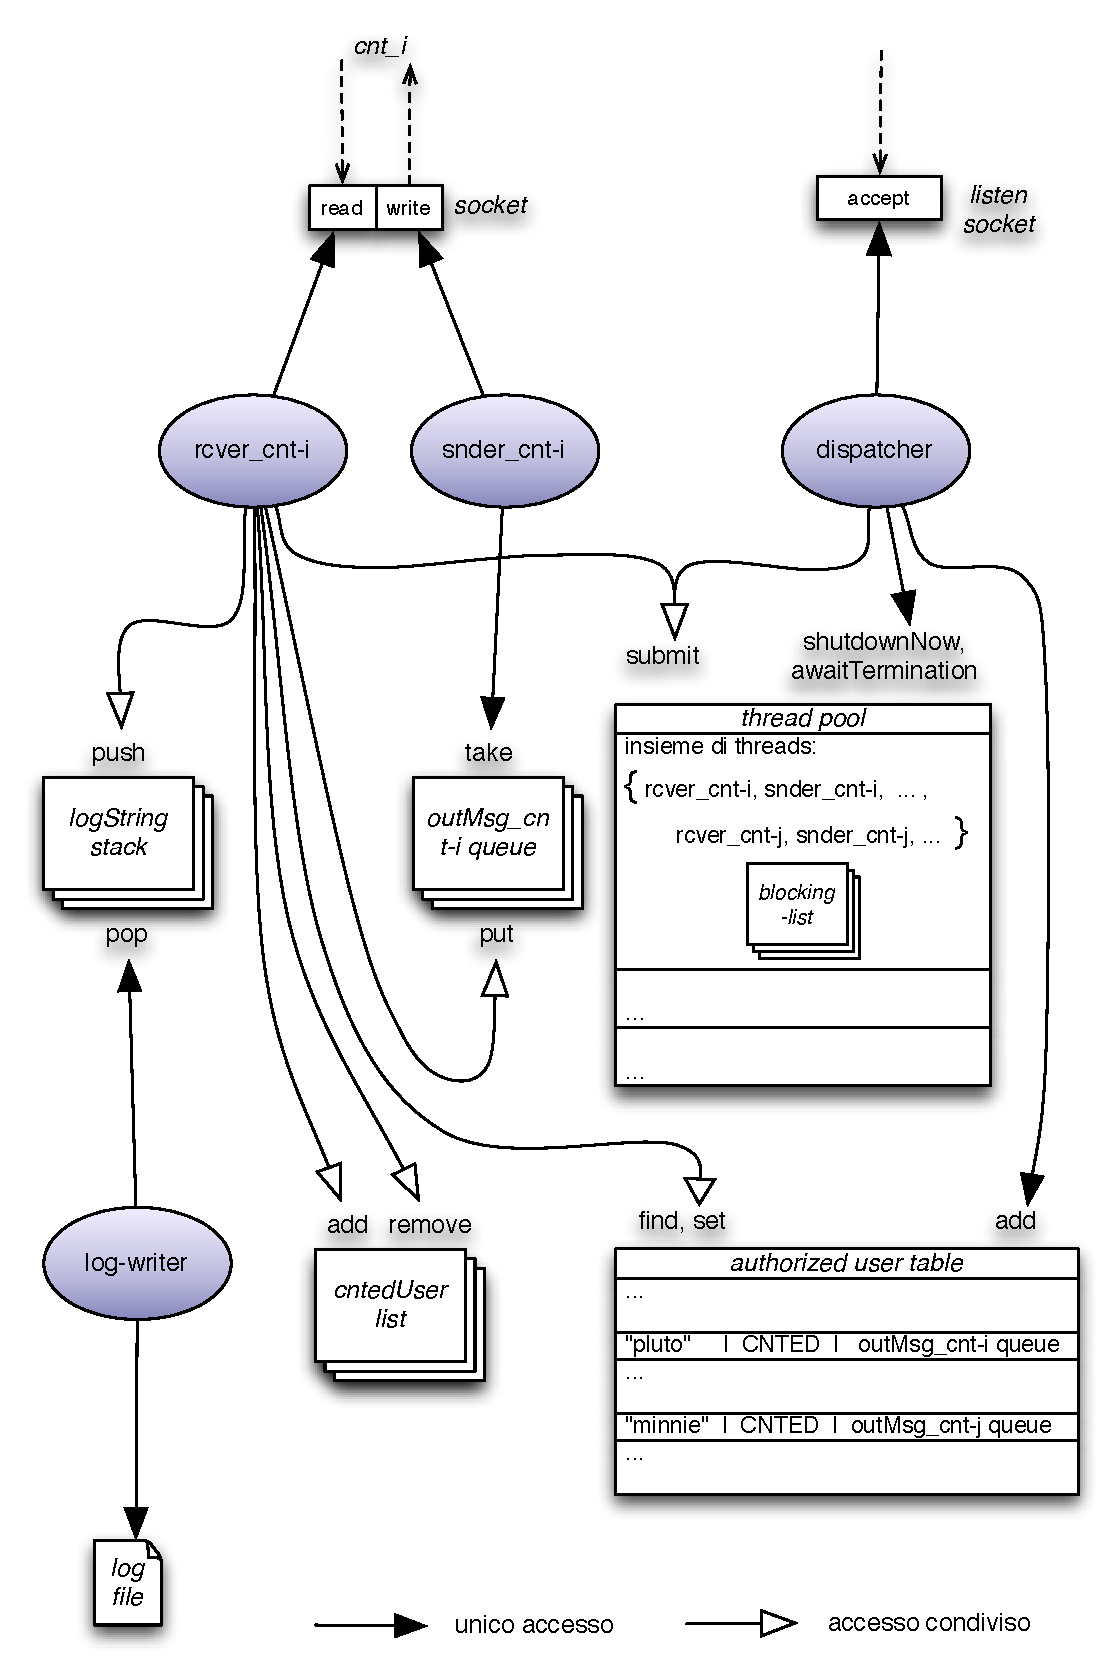
\includegraphics[scale = 0.6]{serverObjects.pdf}
  \caption{Strutture Dati e Threads usati nel processo
    \texttt{msgserv}. Nota: sono mostrati i threads e le strutture
    relativi solo alla connessione cnt-i.}
\end{figure}

\subsection{Gestione dei segnali}
Tutti i worker-thread del processo \texttt{msgserv} e il thread
scrittore sul file di log filtrano tutti i segnali, l'unico thread che
riceve segnali \`e il dispatcher, in tal modo un segnale inviato al
processo \`e ricevuto esclusivamente da tale thread. I segnali sono
usati da tale processo solo per la terminazione, avere un solo punto
di ricezione dei segnali semplifica la gestione della terminazione. Il
thread dispatcher,in fase di inizializzazione, ridefinisce il
comportamento rispetto al segnale \texttt{SIGPIPE} in modo da
ignorarlo ed ai segnali \texttt{SIGINT} e \texttt{SIGTERM} in modo da
impostare al valore 1 la variabile globale \texttt{leave} dichiarata
come \texttt{volatile~sig\-\_atomic\_t}. Tale variabile \`e usata per la
terminazione del processo.

\subsection{Terminazione del processo e dei thread}
La terminazione del processo \texttt{msgserv} avviene unicamente alla
ricezione di un segnale \texttt{SIGINT} o \texttt{SIGTERM} da parte
del thread dispatcher. Come gi\`a enunciato nel paragrafo
\textbf{(3.2)} tutti i thread del processo sono caratterizzati
dall'eseguire un'attivit\`a che per tutta la durata di vita del thread
aspetta una richiesta di un ``cliente'' e la serve. Tale ciclo di vita
ha termine quando la variabile globale \texttt{leave} assume il valore
1 (vero), infatti tale varibile \`e inizializzata a 0 (falso) e viene
modificata solo dal gestore dei segnali di terminazione.

\subsubsection{Terminazione del dispatcher-thread}
Il ciclo di vita di tale thread \`e terminato solo dal valore vero
dalla variabile globale \texttt{leave}. La fase di terminazione di
tale thread prevede, oltre che alla liberazione di risorse, la
richiesta di shutdown al Thread pool e la relativa attesa, la
cancellazione (richiesta di terminazione) del logwriter-thread e la
relativa atesa e la chiusura e unlink del socket.

\subsubsection{Terminazione di un worker-thread}
I worker-thread sia lettori che scrittori appartengono e sono gestiti
dal Thread pool, quindi le modialit\`a in cui di tali thread possono
terminare sono quelle del Thread pool descritte nelle specifiche delle
funzioni \texttt{threadPool\_shutdown*}. In particolare si \`e detto
che il dispatcher-thread usa lo shutdown istantaneo, caratterizzato
dalla cancellazione di tutti i thread del pool. Per garantire il
completamento di eventuali compiti pendenti il task dei thread
riceventi abilita la cancellazione solo durante l'attesa passiva di un
nuovo messaggio, mentre il task dei thread mittenti disabilitano la
cancellazione all'avvio. Quando un worker-thread ricevente prende atto
della richiesta di cancellazione, tra le operazioni di chiusura
(cleanup) interagisce per l'ultima volta con il worker-thread mittente
associato alla sua stessa connessione inviando uno speciale messaggio
\texttt{message\_t} di tipo \texttt{MSG\_exit} il cui significato \`e
appunto terminare l'esecuzione. Dato che tale messaggio \`e inserito
in una coda \textsc{fifo} tutti i messaggi in uscita pendenti saranno
inviati prima della terminazione del thread.

\subsubsection{Terminazione del logwriter-thread}
Anche tale thread abilita la cancellazione solo quando esegue l'attesa
passiva di un nuovo messaggio di log dalla pila bloccante. Le
operazioni successive all'aver verificato la cancellazione consistono,
tra le altre, di scrivere gli eventuali messaggi di log nella pila non
ancora prelevati.

%%%%%%%%%%%%%%%%%%%%%%%%%%%%%%%%%%%%%%%%%%%%%%%%%%%%%%%%%%%%%%%%%%%%%%%%

\section{Struttura del Client}
\subsection{I threads del processo}
Il processo \texttt{msgcli} \`e inizialmente composto da un unico
thread (quello che esegue la funzione main) che invia la richiesta di
connessione al server e aspetta il messaggio di avvenuta connessione
da parte del server. Solo dopo essere connesso al server tale thread
crea un altro thread, che ha il compito di ricevere e stampare i
messaggi ricevuti dal server, e comincia ad eseguire la funzione che
legge da standard input e invia messaggi al server. 

\subsection{Terminazione del processo}
Esistono tre modi in cui il processo pu\`o terminare:

\subsection*{Terminazione richiesta dall'utente}
L'utente pu\`o richiedere la terminazione ed eventuale disconnessione
dal server con il comando \texttt{\%exit} o inviando un segnale di
terminazione. Nel primo caso il thread mittente al server legge da
standard input la richiesta di uscita e esce dal ciclo di
servizio. Nel secondo caso la gestione dei segnali di terminazione
imposta ad 1 il valore della variabile globale \texttt{leave} di tipo
\texttt{volatile~sig\_atomic\_t} ci\`o fa causare nel thread mittente
al server l'uscita dal ciclo di servizio. Il thread mittete al server
dopo l'uscita dal ciclo di servizio invia il messaggio di uscita
\texttt{MSG\_EXIT} al server dopo di che attende la terminazione del
thread ricevente dal server, solo dopo tale tale attesa viene chiuso
il socket collegato al server. Il thread ricevente dal server termina
correttamente quando riceve il messaggio \texttt{MSG\_OK} di conferma
avvenuta disconnessione. 

\subsection*{Terminazione richiesta dal server (disconnessione)}
Il thread ricevente dal server legge il messaggio di disconnessione
del server \texttt{MSG\_EXIT}, in questo caso l'altro thread viene
cancellato e si termina l'esecuzione.

\subsection*{Terminazione dovuta ad un errore di un thread di msgcli}
In entrambi i thread si terminano i cicli di servizio. Per il thread
mittente al server la gestione della terminazione \`e analoga al caso
della terminazione richiesta dall'utente. Per il thread ricevente dal
server la gestione consiste nel cancellare l'altro thread e terminare.

%%%%%%%%%%%%%%%%%%%%%%%%%%%%%%%%%%%%%%%%%%%%%%%%%%%%%%%%%%%%%%%%%%%%%%%%
\appendix
\section{Appendice: Guida per l'utente}

\subsection{Compliazione}
Eseguire \texttt{make} in \verb+PROJ_BASEDIR/src/+ gli argomenti
\emph{msgserv} e \emph{msgcli} per creare i file eseguibili
\texttt{msgserv} e \texttt{msgcli} e compilare tutti i sorgenti e
librerie necessarie.

\subsection{Installazione e disistallazione}
L'installazione causa la compliazione delle librerie degli eseguibili
\texttt{msgserv}, \texttt{msgcli} e la copia di questi, degli headers
pubblici e delle librerie nelle directory specificate. Per
l'installazione eseguire \texttt{make} in \verb+PROJ_BASEDIR/src/+
con l'argomento \emph{install}, gli eseguibili dei programmi server e
client vengono posizionati nella directory \verb+BIN_DIR+ di default
``\verb+../bin+'', gli headers pubblici vengono copiati in
\verb+HEADERS_DIR+ di default ``\verb+../include+'' e le librerie
vengono copiate in \verb+LIB_DIR+ di default ``\verb+../lib+''. Per
installare in directory diverse modificare il file Makefile nella
definizione delle vaiabili \verb+BIN_DIR+, \verb+HEADERS_DIR+,
\verb+LIB_DIR+ oppure eseguire \texttt{make install} con parametri la
definizione delle variabili, ad esempio:
\begin{verbatim}
make install BIN_DIR="/usr/local/bin" 
\end{verbatim}

La disistallazione causa la rimozione di tutti i file copiati nel
sistema con l'installazione. Per la disistallazione eseguire
\texttt{make uninstall} in \texttt{PROJ\_BASEDIR\-/src/}. 

Per rimuovere i file oggetto creati nella compilazione delle librerie
e degli eseguibili eseguire \texttt{make clean}

\subsection{Esecuzione del Server e del Client}
Per eseguire il server occorre disporre di un file
\texttt{userAuthList} con l'elenco dei nomi degli utenti
autorizzati. Quindi eseguire:
\begin{verbatim}
BIN_DIR/msgserv userAuthList logfile 
\end{verbatim}
Al termine dell'esecuzione il file \texttt{logfile} contiene tutti i
messaggi scambiati dagli utenti, pu\`o essere analizzato dallo script
\texttt{logpro} per statistiche.\\Per eseguire un client \`e
sufficente eseguire con un userName autorizzato:
\begin{verbatim}
BIN_DIR/msgcli userName
\end{verbatim}

\section{Appendice: Debug e Test}
Per controllare il corretto funzionamento dei programmi, nei sorgenti
esistono alcune stampe su standard error di valori e informazioni
ritenuti interessanti in fase di sviluppo, tali stampe vengono
effettuate se sono definite particolari macro. Ogni sorgente ha una
specifica macro che abilita la stapa delle informazioni di debug. In
Makefile esistono variabili che dichiarano macro con la relativa
opzione di \texttt{gcc}, inoltre il valore della variabile \texttt{DBG} \`e
presente in tutte le compilazioni. Ad esempio per abilitare il debug
in \texttt{msgserv} eseguire i seguenti comandi:
\begin{verbatim}
make clean
make msgserv DBG=dbg_msgserv
./msgserv userlist logfile
\end{verbatim}
Per compilare ed effettuare tutti i test degli oggetti non richiesti
dal progetto eseguire \texttt{make myTest}
\end{document}

